\chapter{Ausgangsarchitektur}
\label{ch:INITIAL}

\begin{figure}
    \centering
    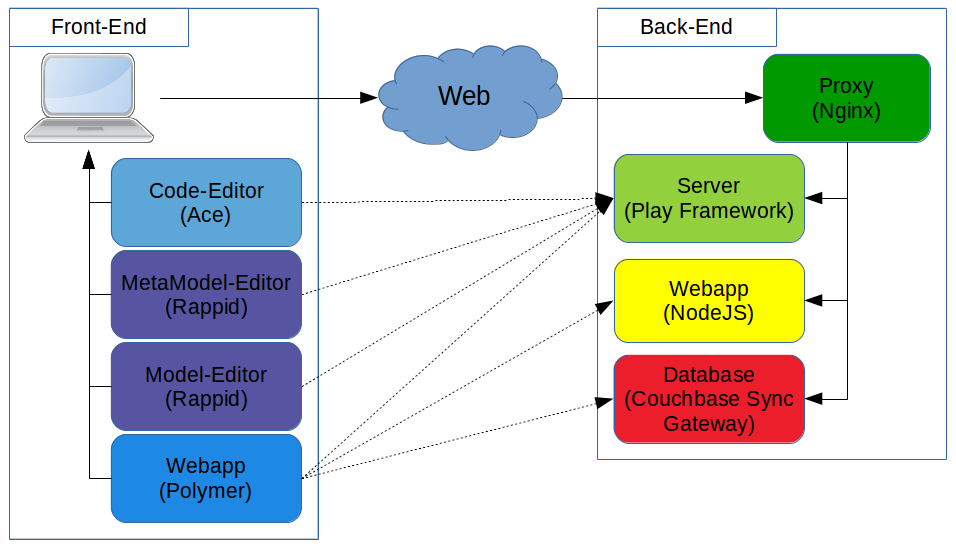
\includegraphics[width=5in]{figures/overview-before.png}
    \caption{Ausgangszustand - Übersicht}
    \label{fig:ZETA_OVERVIEW_OLD}
\end{figure}

Dieses Kapitel beschäftigt sich mit der Beschreibung des Ausgangzustands von \textit{Zeta}. Dabei wird im speziellen auf die Architektur von \textit{Zeta} und ihre Besonderheiten eingegangen. Als Ausgangszustand von \textit{Zeta} wird der Stand aus dem Git-Tag 'AktorSystem-generatorScaling' vom 11.03.2017 \cite{zeta_tag_old} verwendet.

\textit{Zeta} ist eine Webapplikation und besteht aus diesem Grund primär aus einer Client-Server Architektur. Dabei ist der Browser auf dem Computer eines Benutzers in diesem Fall der Client und ein Webserver oder Proxy entsprechend der Server. Dabei wird sämtlicher Code einer Webapplikation der im Client interpretiert und ausgeführt wird im weiteren Verlauf als Front-End und sämtlicher Code der serverseitig ausgeführt wird als Back-End bezeichnet. Eine Übersicht der Client-Server Architektur von \textit{Zeta} wird in Abbildung~\ref{fig:ZETA_OVERVIEW_OLD} auf Seite~\pageref{fig:ZETA_OVERVIEW_OLD} dargestellt. Das Front-End von \textit{Zeta} kommuniziert zentral über einen Reverse Proxy mit dem Back-End. Dabei ist das Front-End in mehrere Unteranwendungen und das Back-End in mehrere Dienste zur eigentlichen Verarbeitung der Anfragen aufgeteilt.

\section{Front-End}
\label{sec:INITIAL_FRONTEND}

Das Front-End umfasst zum einen Teil primär statische Seiten für eine Benutzer-Verwaltung mit Funktionen wie Registrieren, Anmelden und Abmelden. Des Weiteren können neue Projekte angelegt werden. In wenigen Fällen wie im  Beispiel der Projektübersicht oder der Registrierung wird per JavaScript dynamisch auf die Interaktion eines Benutzers reagiert. Die weiteren Teile des Front-Ends umfassen angefangen mit \ac{ria} bis zu \ac{spa} Anwendungen und werden im weiteren Verlauf im Detail betrachtet. Innerhalb eines Projekts wird zuerst ein Modell beschrieben. Dabei wird ein \textit{Code-Editor} zur Definition einiger Teile des Modells per textueller \acp{dsl} benutzt. Darauf folgt der graphische Editor für den \textit{MetaModel-Editor} und den \textit{Model-Editor}. Mit dem \textit{MetaModel-Editor} kann die zugrundeliegende Datenstruktur für die spätere Modell Instanz definiert werden. Aus diesen Informationen kann nun über das Back-End ein \textit{Model-Editor} generiert werden. Dieser \textit{Model-Editor} kommt beim nächsten Schritt zum Anlegen und Bearbeiten von Modell Instanzen zum Einsatz. Als nächstes wird noch die \textit{Webapp} zur Verwaltung von Generatoren benötigt. Dabei werden innerhalb der \textit{Webapp} Transformationsregeln zur \ac{m2t} Transformation angelegt. Aus den Daten der Modell Instanz und den Transformationsregeln kann nun im Back-End über Generatoren schlussendlich jegliche textuelle Form wie z.B. Programmcode in einer beliebigen Programmiersprache erzeugt werden. Im weiteren Verlauf dieses Abschnitts wird noch mal genauer auf die technischen Details des \textit{Code-Editors}, des graphischen Editors für den \textit{MetaModel-} und \textit{Model-Editor} und der \textit{Webapp} eingegangen.

\subsection{Code-Editor}

Wie zuvor erwähnt werden textuelle \acp{dsl} in Teilen zur Beschreibung des Modells genutzt und zu diesem Zweck wird ein \textit{Code-Editor} benötigt. Der \textit{Code-Editor} von \textit{Zeta} ist eine \ac{ria} Anwendung und baut auf den Open Source und selbst ernannten High Performance Code Editor für das Web namens \ac{ace} auf \cite{zeta_ace_html} \cite{zeta_ace_scala}. \ac{ace} ist der primäre Editor der webbasierten \textit{Cloud9 IDE}, welche inzwischen von Amazon unter dem Namen \textit{AWS Cloud9} vertrieben wird \cite{ace_about} \cite{ace_aws}. Die erste Version von \ac{ace} wurde 2010 veröffentlicht und wird bis heute unter anderem von Mozilla gewartet. Die Funktionen von \ac{ace} umfassen unter anderem Syntax-Highlighting mit verschiedenen Themes, automatisches Einrücken, flexible anpassbare Tastaturkürzel, eine Suche, Aus- und Einblenden einzelner Blöcke eines Programmcodes, einen \textit{Live Syntax Checker} und eine einfache Autovervollständigung.

Initial werden die Ressourcen des \textit{Code-Editors} wie \ac{html}-, \ac{css}- und JavaScript-Dateien vom \textit{Play Server} über den \textit{Proxy} Dienst an den Browser eines Benutzers ausgeliefert. Zur Laufzeit  nutzt \textit{Zeta} zur Beschreibung der Grammatik für die einzelnen textuellen \ac{dsl} die Open Source Bibliothek \textit{Ace-Grammar} \cite{ace_grammar}. Dabei wird aus einem \ac{json} Schema ein Syntax-Highlighting Parser für \ac{ace} erzeugt. Zusätzlich verbindet sich der \textit{Code-Editor} über einen Websocket mit dem \textit{Play Server}. Über diesen Websocket wird bei jeder Änderung der aktuelle Inhalt des \textit{Code-Editors} vom Browser an das Back-End übermittelt. Des Weiteren wird aber auch der \textit{Code-Editor} über den Websocket vom Back-End über den initialen und über Änderungen am Inhalt informiert, damit \ac{ace} entsprechend eine neue Sitzung mit dem aktuellen Inhalt und dem Syntax Highlighting Parser erstellt. Mit diesem Mechanismus ist es möglich, kollaborativ mit mehreren Benutzern an den Definitionen einer textuellen \ac{dsl} zu arbeiten, da der Stand zwischen den in mehreren Web Browser geöffeneten \textit{Code-Editoren} synchronisiert wird. Abschließend wird auch bei jeder Änderung des Inhalts im \textit{Code-Editor} noch der aktuelle Stand über einen Webservice des \textit{Play Servers} zusätzlich im Back-End persistiert.

\subsection{Graphischer Editor}

Der \textit{MetaModel-} und \textit{Model-Editor} in \textit{Zeta} ist eine \ac{ria} Anwendung und besteht primär aus einem graphischer Editor. \textit{Zeta} setzt hierbei auf das proprietäre \textit{Rappid Diagramm Framework} oder kurz \textit{Rappid} genannt. Der \textit{Rappid} wird von der Firma \textit{client IO} entwickelt und basiert auf der Open Source Diagramm Bibliothek \textit{JointJS} derselbigen Firma. Während \textit{JointJS} grundlegende Funktionen zur Erstellung von \acp{svg} bietet, erweitert \textit{Rappid} dieses Grundgerüst um einen vollwertigen webbasierten graphischen Editor. Hierbei kann \textit{Rappid} im Browser aus einer Palette einzelner Diagrammelemente per Drag \& Drop neue Elemente auf einer Arbeitsfläche erstellen. \textit{Rappid} unterstützt weiterhin Funktionen wie ein Backroll oder das Wiederholen von Änderungen, Realtime Kollaboration, Export als raster- oder vector-basierter Grafik und einem Inspektor zur erweiterten Bearbeitung der Inhalte eines Diagrammelements.

Der \textit{MetaModel-Editor} in \textit{Zeta} wird zur Definition eines Meta Modells eingesetzt. Dabei werden die Ressourcen für den \textit{MetaModel-Editor} vom \textit{Play Server} über den \textit{Proxy} Dienst an den Browser des Benutzers übermittelt. Der Stand des Editors wird initial beim Laden des Editors per Browser über das \ac{html} Dokument als \ac{json} in einer globalen JavaScript Variable mitgesendet und muss nicht zusätzlich über einen Webservice geladen werden. Zur Laufzeit wird \textit{Rappid} mit den zuvor definierten Diagrammelementen mit entsprechenden Inspektoren und einigen eigens für \textit{Zeta} entwickelten Erweiterungen initialisiert. Eine dieser Erweiterungen z.B. synchronisiert den aktuellen Stand des \textit{MetaModel-Editors} über mehrere im Browser geöffnete Instanzen und ermöglicht somit kollaboratives Arbeiten mehrerer Benutzer an ein und demselben Meta Modell. Eine andere Erweiterung erzeugt beim Speichern aus dem aktuellen Stand die Datenstruktur des Meta Modells und sendet diese zusammen mit weiteren Information des \textit{UI-State} wie z.B. Position, Hintergrundfarbe und etc. einzelner Diagrammelemente über einen Webservice \ac{api} an den \textit{Play Server}.

Der \textit{Model-Editor} wird dazu genutzt, um die Inhalte einer Modell Instanz zu definieren. Auch hier werden die Ressourcen des Editors über den \textit{Play Server} ausgeliefert und auch der initiale Stand des Editors wird über eine globale JavaScript Variable im \ac{html} Dokument mitgeliefert. Während im \textit{MetaModel-Editor} nur zwei Diagrammelemente benötigt werden, muss der \textit{Model-Editor} mit Diagrammelementen auf Basis der Definitionen aus den \textit{Code-Editoren} arbeiten und muss die Inhalte aus den Inspektoren auf die Datenstruktur des Meta Modells mappen. Zu diesem Zweck wird über den \textit{Generate-Button} in der Projektübersicht die Erzeugung von JavaScript Dateien für den \textit{Model-Editor} angestoßen. Anhand der Definition aus dem \textit{Code-Editor} und dem \textit{MetaModel-Editor} werden nun innerhalb des \textit{Play Servers} einzelne JavaScript Dateien zur späteren Konfiguration von \textit{Rappid} im Browser erzeugt. Bei jeder Änderung über den \textit{Code-Editor} oder \textit{MetaModel-Editor} müssen diese JavaScript Dateien erneut erzeugt werden. Auch für den \textit{Model-Editor} wurden eigens für \textit{Rappid} einige Erweiterungen programmiert. Zum Speichern werden wie auch im \textit{MetaModel-Editor} mit einem Exporter aus dem aktuellen Stand des Editors die Daten in ein bestimmtes Schema \ac{json} Schema überführt und zusammen mit dem \textit{UI-State} per Webservice \ac{api} an den \textit{Play Server} zur Persistierung übermittelt. Zusätzlich ist der \textit{Model-Editor} noch an einen Websocket des \textit{Play Servers} angebunden. Dabei wird beim Speichern das Back-End per Websocket über dieses Ereignis informiert und parallel wird der Browser bei Änderungen über die aktuelle Liste an sogenanntem und nicht näher beschriebenem \textit{BondedTask} informiert. Die Liste an \textit{BondedTask} wird im \textit{Model-Editor} dargestellt und per Klick auf einen Eintrag wird das Back-End per Websocket über das Ausführen eines \textit{Bonded-Task} beauftragt. Entsprechend informiert das Back-End den Browser per Websocket über den Start und Abschluss eines \textit{Bonded-Tasks}. Diese \textit{Bonded-Tasks} können nicht im \textit{Model-Editor} erstellt werden, sondern werden über die \textit{Webapp} erzeugt.

\subsection{Webapp}

Die \textit{Webapp} ist eine \ac{spa} mit entsprechend clientseitigem Routing und wird parallel neben dem \textit{Play Server} über einen \textit{Node.js} Server ausgeliefert. Die \textit{Webapp} basiert auf der \textit{Polymer} Bibliothek für Web Components. \textit{Polymer} wird von Google entwickelt und wurde unter anderem beim Redesign von \textit{Youtube} eingesetzt. Die \textit{Webapp} von \textit{Zeta} bietet zum einen eine Oberfläche zur Erstellung bzw. zum Anpassen eines Generators mit seinen \ac{m2t} Transformationsregeln. Zum anderen können die Generatoren gestartet und gestoppt werden. Zusätzlich können die erstellten Generatoren noch über programmierbare Filter gruppiert werden. Aufbauend auf den Generatoren und den Filtern können noch verschiedene Task wie z.B. einen \textit{Bonded-Task} oder einen \textit{Timed-Task} erstellt werden.

Dabei ist die \textit{Webapp} größtenteils unabhängig von Back-End und nutzt nur einen einzigen Websocket, um mit dem \textit{Play Server} zu kommunizieren. Über den Websocket auf der \ac{url} \textit{/socket/developer} wird der Browser zum einen in regelmäßigen Abständen über laufende Generatoren informiert und zum anderen über die Ausgaben des einzelnen Generators. Die \textit{Webapp} beauftragt wiederum das Back-End über den Websocket z.B. das Starten oder Stoppen eines Generators. Zum Teil persistieren die Generatoren während ihrer Ausführung die Daten selbstständig zum \textit{Couchbase Sync Gateway}. Die restlichen Daten werden clientseitig im Browser zum \textit{Couchbase Sync Gateway} persistiert. Dabei greift die \textit{Webapp} nicht direkt, sondern entsprechend über den \textit{Proxy} Dienst auf das \textit{Sync Gateway} zu. Die notwendige Sitzung für die Authentifizierung am \textit{Sync Gateway} wurde zuvor bei der Anmeldung des Benutzers am \textit{Play Server} initiiert. Des Weiteren ist die \textit{Webapp} über ein Websocket an einen \textit{Live Change Feed} des \textit{Sync Gateways} angeschlossen. Falls nun Dokumente der Datenbank über das \textit{Sync Gateway} angepasst werden, wird die \textit{Webapp} über diese Änderung informiert und aktualisiert entsprechend die vorgehaltenen Daten.

\section{Back-End}

Das Back-End von \textit{Zeta} besteht aus einer Reihe von auf ihren Anwendungsfall spezialisierten Diensten. Jeder Dienst wird isoliert von den anderen Diensten des Betriebssystems und den einzelnen Diensten von \textit{Zeta} in einem \textit{Docker Container} ausgeführt. Dabei sind die verschiedenen \textit{Docker Container} bei \textit{Zeta} zu einem Verbund zusammengefasst. Dieser Verbund ist per \textit{Docker Compose} definiert \cite{zeta_docker_compose}. Eine Übersicht dieser Dienste mit ihren Kommunikationskanälen können in Abbildung~\ref{fig:ZETA_ARCH_OLD} auf Seite~\pageref{fig:ZETA_ARCH_OLD} eingesehen werden. Dabei wird in der Abbildung zwischen den initial gestarteten Containern von \textit{Docker Compose} und den Containern des \textit{Docker Compose} Netwerks unterschieden, da \textit{Zeta} zur Laufzeit je Generator einen Container über den \textit{Docker Daemon} startet und diesen zusätzlich dem Netzwerk der \textit{Docker Compose} Instanz beitreten lässt. Die \textit{Docker Container} der Generatoren müssen dem \textit{Docker Compose} Netzwerk von \textit{Zeta} beitreten, da das private Netzwerk der \textit{Docker Compose} Instanz nur ganz gezielt externen Zugriff zulässt und die Generatoren einen Zugriff auf den einen oder anderen Dienst von \textit{Zeta} benötigen.

\begin{figure}
    \centering
    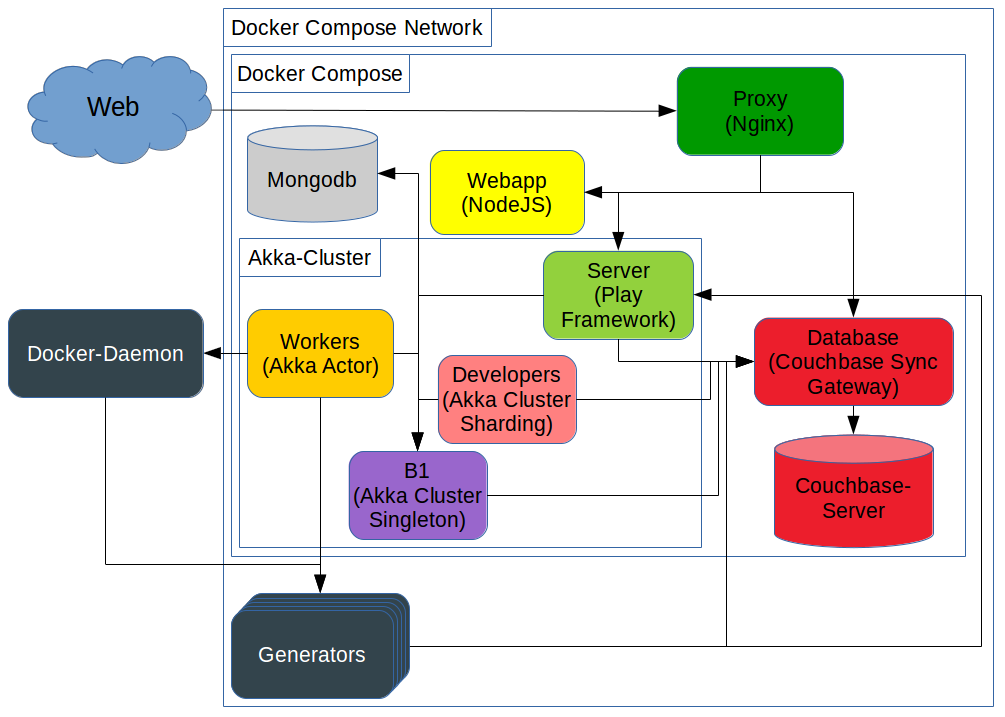
\includegraphics[width=5in]{figures/docker-compose-before.png}
    \caption{Ausgangszustand - Dienste}
    \label{fig:ZETA_ARCH_OLD}
\end{figure}

Auf der höchsten Ebene der Dienste fungiert im Back-End von \textit{Zeta} ein \textit{Nginx} Server als Reverse Proxy und ist somit die öffentliche \ac{api} für sämtliche Anfragen der Benutzer aus dem \ac{www}. Von dem Reverse Proxy aus werden die Anfragen entsprechend der genutzten \ac{url} an den \textit{Webapp} Dienst, das \textit{Couchbase Sync Gateway} oder den \textit{Play Server} verteilt. Der \textit{Webapp} Dienst ist ein auf \textit{Node.js} basierender Webserver und seine primäre Aufgabe ist es, die Ressourcen der \textit{Webapp} auszuliefern. Zusätzlich fungiert die Erweiterung \textit{Browsersync} als Proxy innerhalb des \textit{Webapp} Diensts und umfasst unter anderem Funktionen wie automatischer Pagereload bei Änderungen am Programmcode der \textit{Webapp} oder synchronisiertes Ausführen von Scroll und Klick Events über mehrere Browser Instanzen. \textit{Browsersync} wird hauptsächlich zu Testzwecken z.B. von verschiedenen Geräten auf Entwicklersystemen eingesetzt. Als zweites leitet der Reverse Proxy die Anfragen an die \ac{rest} \ac{api} oder die Websockets des \textit{Couchbase Sync Gateways} weiter. Zum einen fungiert das \textit{Sync Gateway} als Proxy zu einem Cluster aus einem oder mehreren \textit{Couchbase Servern} und zusätzlich wird z.B. über den \textit{Sync Endpoint} per Websocket ein \textit{Change Feed} zur Verfügung gestellt. Als letztes werden die Anfragen noch an den \textit{Play Server} weitergeleitet. Der \textit{Play Server} basiert auf dem in Scala geschriebenen \textit{Play Web Framework} und ist die ehemalige Kernkomponente von \textit{Zeta}. Der \textit{Play Server} umfasst eine Reihe an unterschiedlichen Funktionalitäten und ist nur ein Unterprojekt unter mehreren innerhalb eines größeren Scala Projekts. Zum einen bietet der \textit{Play Server} die webbasierte Oberfläche zur Benutzer- und Projektverwaltung, den \textit{Code-Editor}, den \textit{MetaModel-} und \textit{Model-Editor}. Zum anderen bietet er eine Reihe von Webservice \acp{api} und Websockets an. Dabei werden im Besonderen einige Anfragen der Websockets zu den Microservices zur Generatorverwaltung innerhalb des \textit{Akka Clusters} weitergereicht.

Im weiteren Verlauf dieses Abschnitts wird zuerst auf das Build System von \textit{Zeta} eingegangen. Dabei wird zum einen der Build Vorgang der eigens für \textit{Docker Compose} erzeugten \textit{Docker Images} betrachtet und zum anderen die Konfiguration von \ac{sbt} für die einzelnen Unterprojekte des Scala Projekts. Danach folgt eine genauere Betrachtung der Webservice \ac{api} und Websockets des \textit{Play Server} und der Teilkomponenten des \textit{Play Servers} wie dem \textit{SprayParser} mit seiner Notwendigkeit für die drei textuellen \acp{dsl}. Weitergehend werden die Aufgaben des \textit{Akka Clusters} mit der \ac{m2t} Transformation betrachtet. Abschließend wird die Rolle der \textit{Mongodb} und des \textit{Couchbase Servers} mit seinem \textit{Sync Gateway} im Detail beschrieben.

\subsection{Build-System}
\label{sec:INITIAL_BUILD}

\begin{figure}
    \centering
    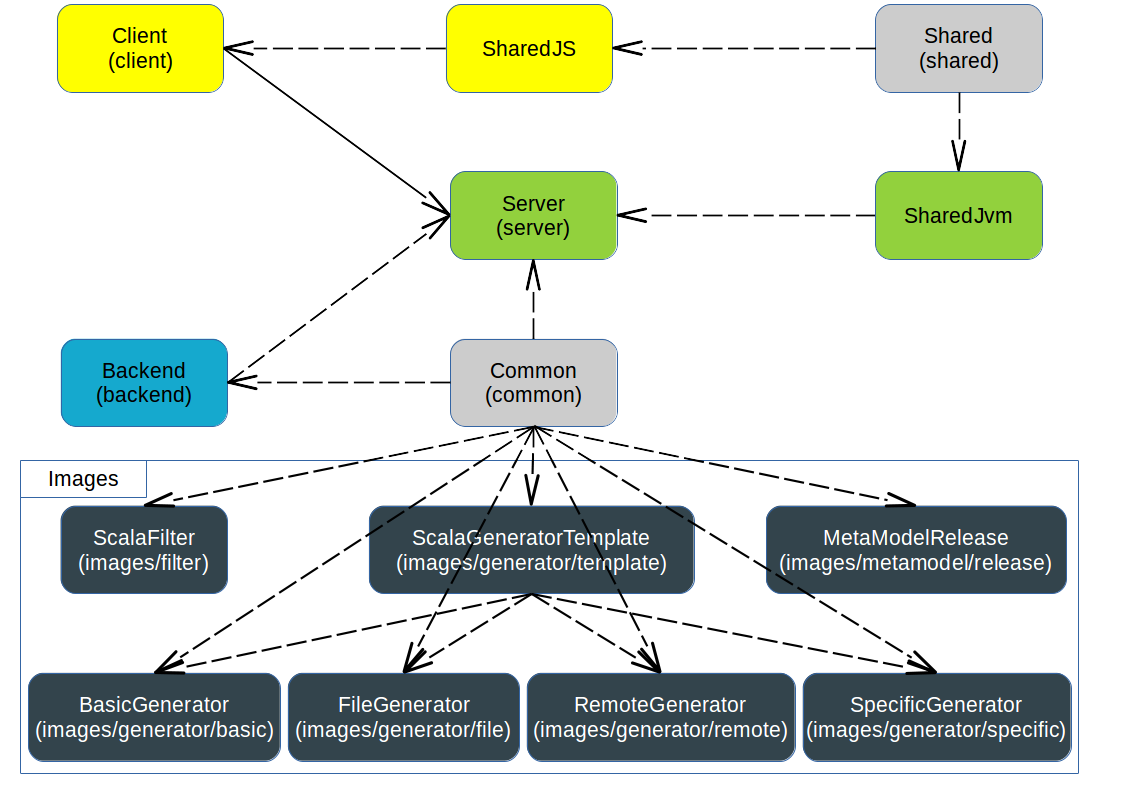
\includegraphics[width=5in]{figures/sbt-modules-before.png}
    \caption{Ausgangszustand - SBT Unterprojekte}
    \label{fig:ZETA_SBT_OLD}
\end{figure}

In diesem Unterabschnitt geht es zuerst um den Build Vorgang für die \textit{Docker Images} der einzelnen Dienste von \textit{Zeta} und darauf folgt ein tieferer Einblick in die \ac{sbt} Konfiguration des Scala Projekts. Die Laufzeitumgebung für ganz \textit{Zeta} mit den verschiedenen Diensten ist über \textit{Docker Compose} definiert \cite{zeta_docker_compose}. Für die einzelnen Dienste werden auf ihre Laufzeitumgebung optimierte \textit{Docker Images} verwendet. Dabei sind die \textit{Docker Images} nicht von Grund auf neu definiert, sondern erweitern schon bestehende öffentliche \textit{Docker Images}. Bevor die Container für die einzelnen Dienste gestartet werden können, müssen die Images in einem Build Vorgang von \textit{Docker} erzeugt werden. Dieser Vorgang wird automatisch von \textit{Docker Compose} beim Starten ausgeführt, falls die \textit{Docker Images} nicht vorhanden sind oder die genutzten Dateien für das Image sich geändert haben. Der \textit{Proxy} Dienst baut auf dem offiziellen Image für \textit{Nginx} auf und fügt zusätzlich noch eine Konfigurationsdatei zur Weiterleitung des Traffic an den entsprechenden Dienst hinzu. Der Zugriff auf diese Dienste wird beim Starten des Containers über sogenannte Links ermöglicht. Zusätzlich wird noch der Standard Port für \ac{http} des Webservers öffentlich für alle Netzwerkschnittstellen freigegeben. Beim Image für den \textit{Couchbase Server} Dienst wird auch auf dem offiziellen Image aufgebaut. Dabei wird der reguläre \textit{ENTRYPOINT} des Image mit einem eigenen ausgetauscht. Dieser neue \textit{ENTRYPOINT} erweitert den regulären \textit{ENTRYPOINT} mit der Funktionalität beim ersten Start eine Datenbank mit einem Benutzer und Passwort zu erstellen. Zur Laufzeit des \textit{Docker Containers} werden noch der Name der Datenbank, der Benutzer und das Password übergeben und einige Ports des \textit{Couchbase Servers} für den öffentlichen Zugriff freigegeben. Alle Dateien eines \textit{Docker Containers}, die zur Laufzeit erstellt worden sind, werden beim Löschen des Containers entfernt und aus diesem Grund wird der Ordner mit Daten der Datenbank per \textit{Bind Mount} persistiert. Beim \textit{Database} Dienst baut das Image auf dem offiziellen \textit{Sync Gateway} Image von Couchbase auf. Dabei wird für das Image eine eigene Konfigurationsdatei zum \textit{Couchbase Server} und ein \textit{ENTRYPOINT} hinzugefügt. Der eigene \textit{ENTRYPOINT} wartet zu Beginn auf die Erreichbarkeit des \textit{Couchbase Servers} und startet anschließend das \textit{Sync Gateway} mit dem Pfad zur eigenen Konfigurationsdatei. Beim \textit{Webapp} Dienst wird beim Image entsprechend auf dem  offiziellen \textit{Node.js} Image aufgebaut. Für das Image kommt zuerst \ac{npm} zum Auflösen der Abhängigkeiten wie den Webserver für \textit{Polymer}, die \textit{Browsersync} Erweiterung und \textit{Bower} zum Einsatz. Nachfolgend wird noch \textit{Polymer} mit seinen Abhängigkeiten per \textit{Bower} heruntergeladen. Zum Schluss wird einmal der gesamte Programmcode der \textit{Webapp} in das Image kopiert. Zur Laufzeit wird zusätzlich nochmal der gesamte Programmcode der \textit{Webapp} in den Container per \textit{Bind Mount} gemapped und die Ordner mit den heruntergeladenen Abhängigkeiten auf ein Volume gemapped. Auch für den \textit{Webapp} Dienst werden verschiede Ports des Webservers und des \textit{Browsersync} Proxys für den öffentlichen Zugriff freigegeben. Für den \textit{Mongodb} Dienst wird nur das offizielle Image benutzt und kein eigenes. Zur Laufzeit wird der Port des \textit{Mongodb} Servers freigegeben und die Daten per \textit{Bind Mount} persistiert. Für die weiteren Dienste wie dem des \textit{Play Servers} werden auch eigene Docker Images benötigt, doch diese werden nicht von \textit{Docker Compose} erzeugt, sondern müssen zuvor über ein Setupscript per \ac{sbt} wie im Programmcode~\ref{lst:ZETA_SETUP} auf Seite~\pageref{lst:ZETA_SETUP} erzeugt werden. Innerhalb dieses Setupscript wird neben den \textit{Docker Images} der \ac{sbt} Unterprojekte noch ein Image zum initialen Befüllen der Datenbank über ein \textit{Node.js} Script erzeugt. Nachdem die Datenbanken von \textit{Docker Compose} gestartet worden sind, muss einmalig ein \textit{Docker Container} mit diesem Image gestartet werden.

\bigskip
\begin{lstlisting}[caption={[Zeta Setupscript]Zeta Setupscript \cite{zeta_setupscript}},label={lst:ZETA_SETUP}]
pushd api
sbt 'project backend' 'docker:publishLocal'
sbt 'project server' 'docker:publishLocal'
sbt 'project scalaFilter' 'docker:publishLocal'
sbt 'project basicGenerator' 'docker:publishLocal'
sbt 'project fileGenerator' 'docker:publishLocal'
sbt 'project specificGenerator' 'docker:publishLocal'
sbt 'project remoteGenerator' 'docker:publishLocal'
popd

docker-compose build

pushd data
docker build -t modigen:data .
popd
\end{lstlisting}
\smallskip

Der \textit{Play Server} ist wie zuvor erwähnt nur eines von mehreren Unterprojekten innerhalb eines Scala Projekts und eine Übersicht aller Scala Unterprojekte mit ihrena Abhängigkeiten untereinander kann in Abbildung~\ref{fig:ZETA_SBT_OLD} auf Seite~\pageref{fig:ZETA_SBT_OLD} eingesehen werden. Dabei steht unterhalb jedes Unterprojekts der entsprechende Ordner innerhalb des Scala Projekts. \textit{Zeta} nutzt \ac{sbt} für den Build Vorgang des Scala Projekts. \ac{sbt} ist ein Buildtool für Java, Scala und mehr \cite{sbt}. Die Funktionalitäten von \ac{sbt} umfassen zum einen das Auflösen der zuvor definierte \ac{sbt} Version und die Abhängigkeiten der verschiedenen Scala Unterprojekte von Zeta \cite{zeta_api_built}. Zum anderen kann \ac{sbt} noch durch sogenannte Plugins erweitert werden. Eine Liste der genutzten Plugins für \textit{Zeta} kann in der Tabelle~\ref{tab:ZETA_SBT_OLD} auf Seite~\pageref{tab:ZETA_SBT_OLD} gefunden werden. Die ersten beiden \ac{sbt} Plugins namens \textit{sbt-revolver} und \textit{sbt-scalariform} sollen allgemein die Entwicklung unterstützen. Das nächste \ac{sbt} Plugin ist primär für die Einbindung des \textit{Play Frameworks} in \ac{sbt} zuständig. Neben einigen Funktionalitäten zur Vereinfachung der Entwicklung, baut es auch auf \textit{SbtWeb} auf. \textit{SbtWeb} ist für die Verwaltung und Auflösung von Assets zuständig und war ursprünglich Teil des \textit{Play Frameworks} \cite{sbtweb}. Zusätzlich erkennt \textit{SbtWeb} noch \textit{WebJars}. \textit{WebJars} enthalten den Programmcode bekannter Frontend Bibliotheken, wie z.B. \textit{jQuery} oder auch \textit{Bootstrap}, und können als reguläre Abhängigkeit per \ac{sbt} zu einem Scala Projekt hinzugefügt werden. Neben den \textit{WebJars} enthält der \textit{Play Server} von \textit{Zeta} noch Kopien einiger der genutzten JavaScript Bibliotheken wie z.B. \ac{ace} oder auch \textit{Rappid}. Mit \textit{SbtWeb} werden zur Laufzeit des \textit{Play Server} der Inhalt der \textit{WebJars} sowie die weiteren Dateien von Assets über den Webserver öffentlich zur Verfügung gestellt. Bei den sogenannten Assets handelt es sich bei \textit{SbtWeb} um Ressourcen für den Browser wie z.B. Datei mit JavaScript, \ac{css} oder auch um Bilder. Damit \textit{SbtWeb} die Existens dieser Assets erkennen kann, müssen diese in entsprechenden Ordnern vorhanden sein. Alle weiteren \ac{sbt} Plugins für \textit{Zeta} erweitern nur noch die Funktionalität von \textit{SbtWeb}, wie z.B. das \textit{sbt-cofffeescript} Plugin als CoffeeScript zu JavaScript Compiler.

\begin{table}[ht]
    \smallskip
    \centering
    \begin{tabular}{| l | l | c | l |}
    \hline
    \bf GroupID & \bf ArtifactID & \bf SbtWeb & \bf Beschreibung \\ \hline
    io.spray & sbt-revolver & & Restart bei Änderung \\ \hline
    org.scalariform & sbt-scalariform & & Programmcode Formatierung \\ \hline
    com.typesafe.play & sbt-plugin & \checkmark & Dev Featues für Play \\ \hline
    com.typesafe.sbt & sbt-coffeescript & \checkmark & CoffeeScript Compiler  \\ \hline
    com.typesafe.sbt & sbt-gzip & \checkmark & Gzipped Web Assets \\ \hline
    com.vmunier & sbt-play-scalajs & \checkmark & ScalaJS für Play Framework\\ \hline
    org.scala-js & sbt-scalajs & & ScalaJS \\ \hline
    \end{tabular}
    \caption{Ausgangszustand - SBT Plugins \cite{zeta_sbt_plugins}}
    \label{tab:ZETA_SBT_OLD}
\end{table}

Wie in der Abbildung~\ref{fig:ZETA_SBT_OLD} auf Seite~\pageref{fig:ZETA_SBT_OLD} zusehen, hängt der \textit{Play Server} von einigen anderen Unterprojekten ab. Eines davon ist das \textit{Client} Projekt. Das \textit{Client} Projekt baut auf \textit{ScalaJS} und dem \textit{sbt-play-scalajs} Plugin zur Zusammenarbeit zwischen \textit{ScalaJS} und dem \textit{Play Framework} auf. Alle \textit{ScalaJS} Projekte sind in der Abbildung~\ref{fig:ZETA_SBT_OLD} auf Seite~\pageref{fig:ZETA_SBT_OLD} mit einer grauen Hintergrundfarbe markiert. Die Aufgabe von \textit{ScalaJS} ist es, als Scala zu JavaScript Compiler zu fungieren. Innerhalb von \textit{ScalaJS} können schon bestehende JavaScript Bibliotheken wie z.B. \textit{jQuery} genutzt werden. Damit während des Build Prozesses die Referenzen zu der \acp{api} der in JavaScript geschriebenen Bibliotheken aufgelöst werden können, müssen sogenannte \textit{Facades} vorhanden sein. Die \textit{Facades} bieten einen Mechanismus um die nicht vorhandenen Typ Informationen für die JavaScript Bibliotheken innerhalb von Scala zu definieren. Für ein paar der bekannteren JavaScript Bibliotheken wie z.B. \textit{jQuery} werden Pakete mit den Typ Informationen für \textit{ScalaJS} angeboten. Dabei enthalten diese Pakete aber nicht den Programmcode der JavaScript Bibliotheken. Sondern dieser muss noch z.B. über \textit{WebJars} in das \textit{Play Framework} eingebunden werden. Eingebunden wird das \textit{Client} Projekt in den \textit{Play Server} über die \textit{Pipeline Stages} von \textit{SbtWeb} und einer Reference als \textit{ScalaJS} Projekt. Dabei kann über die \textit{Pipeline Stages} von \textit{SbtWeb} noch die Form des generierten JavaScript zwischen einer stark optimierten Variante für den Produktivbetrieb oder einer deutlich lesbareren Variante für ein Entwicklersystem entschieden werden. Inhaltlich geht es bei \textit{Client} Projekt um die Konfiguration und Initialisierung des \textit{Code-Editors} und die eigentliche Einbindung erfolgt dabei, wie in Programmcode~\ref{lst:PLAY_CODE_EDITOR} auf Seite~\pageref{lst:PLAY_CODE_EDITOR} zusehen, innerhalb eines Templates im \textit{Play Server}.

\bigskip
\begin{lstlisting}[caption={[Lade und initialisiere Client]Lade und initialisiere Client \cite{zeta_load_client}},label={lst:PLAY_CODE_EDITOR}]
@playscalajs.html.selectScript("client", "/assets")

<script type="text/javascript">
  client.Main().main("@uuid", "@dslType");
</script>
\end{lstlisting}
\smallskip

Das \textit{Client} Projekt besitzt zusätzlich noch als einziges Scala Projekt eine interne Abhängigkeit auf das \textit{SharedJS} Projekt. Dabei ist das \textit{SharedJS} Projekt ein \textit{ScalaJS} Projekt und zusätzlich kein vollwertiges \ac{sbt} Projekt im eigentlichen Sinn. Stattdessen wird das \textit{SharedJS} Projekt aus dem \textit{Shared} Projekt erzeugt. Das \textit{Shared} Projekt wiederrum ist ein sogenanntes \textit{CrossProject} und ermöglicht es, dieselbe Codebase zum einen als \textit{ScalaJS} Projekt und zum anderen als ein reguläres \ac{sbt} Projekt als Abhängigkeit einzubinden. Aus diesem Grund werden aus dem \textit{Shared} Projekt die beiden Projekte \textit{SharedJS} und \textit{SharedJvm} erzeugt. Das \textit{SharedJvm} Projekt wird wiederum vom \textit{Play Server} als Abhängigkeit eingebunden. Das \textit{Shared} Projekt besteht nur aus zwei Scala Dateien und diese beinhalten zum einen das Kommunikationsobjekte für den Websocket des \textit{Code-Editors} und den Actor für das sogenannte \textit{DataVis} Feature des \textit{Model-Editors}.

Während die oberen Projekte auf der Abbildung~\ref{fig:ZETA_SBT_OLD} auf Seite~\pageref{fig:ZETA_SBT_OLD} primäre dem \textit{Play Server} zuarbeiten, handelt es sich bei den unteren Projekten um die späteren Generatoren. Dabei benötigen diese Unterprojekte sowie das Back-End Projekt keine \ac{sbt} Plugins. Diese Generatoren werden zur Laufzeit als \textit{Docker Container} vom \textit{Akka Cluster} des Back-End Projekts gestartet und verwenden dazu die zuvor erzeugten \textit{Docker Images}. Innerhalb der Generatoren werden die zuvor über die \textit{Webapp} erstellten und in Scala geschriebenen Transformationsregeln zur \ac{m2t} Transformation ausgeführt. Dazu werden die Transformationsregeln über die \textit{Toolbox} des Scala Compilers geparst, kompiliert und schlussendlich ausgeführt.

\subsection{Webservice API}

Für das Meta Modell und dem Modell werden von \textit{Play Server} entsprechend der Operationen zum Erstellen, Ändern, Löschen oder Auflisten \ac{rest} \acp{api} bereitgestellt. Eine Liste der verschiedenen \ac{rest} Endpoints für das Meta Modell kann in der Tabelle~\ref{tab:ZETA_REST_META_MODEL_OLD} auf Seite~\pageref{tab:ZETA_REST_META_MODEL_OLD} eingesehen werden. Für das Modell sind die verschiedenen Endpoints in der Tabelle~\ref{tab:ZETA_REST_MODEL_OLD} auf Seite~\pageref{tab:ZETA_REST_MODEL_OLD} zu finden. Dabei sind in den Tabellen die innerhalb von \textit{Zeta} genutzten Endpoints grün und die ungenutzten Endpoints mit rot markiert. Die \ac{rest} \ac{api} verwendet für die Ein- und Rückgabe jeweils eigene \ac{json} Schemata. Dabei kommen aufseiten des \textit{Play Servers} Formatierer, zur Umwandlung des internem Modells zum \ac{json} Schema und wieder zurück, zum Einsatz.

\begin{table}[ht]
    \smallskip
    \centering
    \begin{tabular}{| l | l |}
    \hline
    \bf Method & \bf Route \\ \hline
    \colorbox{red}{GET},\colorbox{LimeGreen}{POST} & /metamodels \\ \hline
    \colorbox{red}{GET},\colorbox{red}{PUT},\colorbox{LimeGreen}{DELETE} & /metamodels/\emph{:id} \\ \hline
    \colorbox{LimeGreen}{GET},\colorbox{LimeGreen}{PUT} & /metamodels/\emph{:id}/definition \\ \hline
    \colorbox{LimeGreen}{GET} & /metamodels/\emph{:id}/definition/mclasses \\ \hline
    \colorbox{LimeGreen}{GET} & /metamodels/\emph{:id}/definition/mreferences \\ \hline
    \colorbox{red}{GET} & /metamodels/\emph{:id}/definition/mclasses/\emph{:name} \\ \hline
    \colorbox{red}{GET} & /metamodels/\emph{:id}/definition/mreferences/\emph{:name} \\ \hline
    \colorbox{red}{GET},\colorbox{LimeGreen}{PUT} & /metamodels/\emph{:id}/shape \\ \hline
    \colorbox{red}{GET},\colorbox{LimeGreen}{PUT} & /metamodels/\emph{:id}/style \\ \hline
    \colorbox{red}{GET},\colorbox{LimeGreen}{PUT} & /metamodels/\emph{:id}/diagram \\ \hline
    \end{tabular}
    \caption{Ausgangszustand - Rest Meta Modell Endpoints}
    \label{tab:ZETA_REST_META_MODEL_OLD}
\end{table}

Neben der \ac{rest} \ac{api} wird über einen weiteren Endpoint für jedes, über die Oberfläche angelegte, Projekt noch eine Reihe, von zuvor generierten, JavaScript Dateien zur Verfügung gestellt. Diese Dateien sind zur Konfiguration des graphischen Editors einer Modell Instanz notwendig. Die Konfiguration basiert auf den zuvor per \textit{Code-} und \textit{MetaModel-Editor} erstellten Definitionen aus dem Modell des Projekts. Zu diesem Zweck werden innerhalb des \textit{Play Server} diese Definitionen geparst und über einen internen Generator die einzelnen JavaScript Dateien erzeugt. Dabei muss die Erzeugung der JavaScript Dateien initial und bei jeder Änderung am Modell von Hand über den \textit{Generate-Button} in der Projektübersicht angestoßen werden.

\begin{table}[ht]
    \smallskip
    \centering
    \begin{tabular}{| l | l |}
    \hline
    \bf Method & \bf Route \\ \hline
    \colorbox{red}{GET},\colorbox{LimeGreen}{POST} & /models \\ \hline
    \colorbox{LimeGreen}{GET},\colorbox{red}{PUT},\colorbox{LimeGreen}{DELETE} & /models/\emph{:id} \\ \hline
    \colorbox{red}{GET},\colorbox{LimeGreen}{PUT} & /models/\emph{:id}/definition \\ \hline
    \colorbox{red}{GET} & /models/\emph{:id}/definition/nodes \\ \hline
    \colorbox{red}{GET} & /models/\emph{:id}/definition/nodes/\emph{:name} \\ \hline
    \colorbox{red}{GET} & /models/\emph{:id}/definition/edges \\ \hline
    \colorbox{red}{GET} & /models/\emph{:id}/definition/edges/\emph{:name} \\ \hline
    \end{tabular}
    \caption{table}{Ausgangszustand - Rest Modell Endpoints}
    \label{tab:ZETA_REST_MODEL_OLD}
\end{table}

\subsection{Websockets}

Um für bestimmte Anwendungsfälle für den \textit{Code-}, \textit{MetaModel-}, \textit{Meta-Editor} oder die Generator Verwaltung in der \textit{Webapp} in Echtzeit über Veränderungen informiert zu werden, bietet \textit{Zeta} über eine Reihe von Endpoints im \textit{Play Server} Websockets an. Dabei werden die Websockets im \textit{Play Server} per \textit{Akka Actoren} implementiert, um eine bidirektionale Kommunikation und eine asynchronen Workflow während der offenen Socket Verbindung zu ermöglichen. Wie in Abbildung~\ref{fig:ZETA_WS_OLD} auf Seite~\pageref{fig:ZETA_WS_OLD} dargegestellt lassen sich die Websockets grob in zwei Kategorien einteilen. Die Actoren der oberen Websockets sind Teil des Back-End Projekts und kommunizieren mit dem \textit{Akka Cluster} der Generatoren. Die Actoren der unteren Websockets sind wiederum Teil des \textit{Play Servers} und ermöglichen so z.B. eine Synchronisation desselben Stands eines über mehrere Browser geöffneten \textit{Code-Editors}. Somit lässt sich kollaboratives Arbeiten für den \textit{Code-Editor} über einen Websocket ermöglichen. Des Weiteren wird auch für den graphischen Editor des Meta Modells ein Mechanismus zum kollaborativen Arbeiten über einen Websocket bereitgestellt. Abschließend wird der letzte Websocket des \textit{Play Server} im graphischen Editor für die Modell Instanz zur Aktualisierung eines sogenannten \textit{DataVis-Editors} genutzt, wobei diese Funktion zum Zeitpunkt der Betrachtung in der Oberfläche des \textit{Model-Editors} nicht mehr genutzt wurde.

\begin{figure}
    \centering
    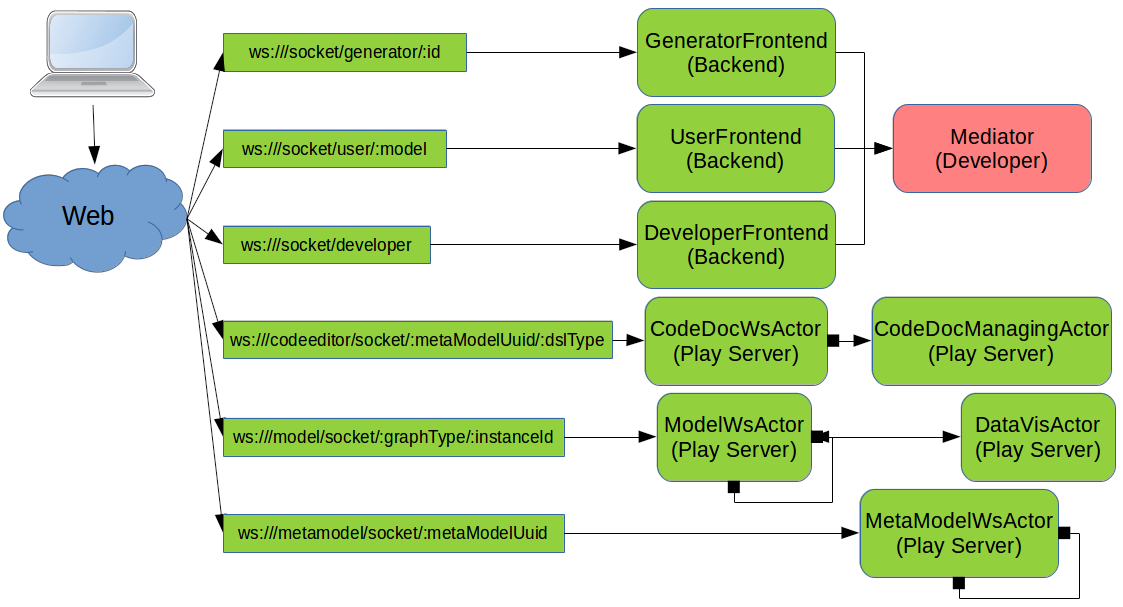
\includegraphics[width=5in]{figures/actor_play_before.png}
    \caption{Ausgangszustand - Websockets}
    \label{fig:ZETA_WS_OLD}
\end{figure}

\subsection{SprayParser}

Der \textit{SprayParser} ist Teil des \textit{Play Servers} und ist verantwortlich dafür die Definitionen der textuellen \acp{dsl} aus dem \textit{Code-Editor} in ein internes Modell zu überführen. Dieses Modell wird genutzt um in einem internen Generator die Konfiguration in JavaScript für den graphischen Editor der Modell Instanzen zu erzeugen. Die Klasse des \textit{SprayParser} besteht im Wesentlichen aus drei verschiedenen aufeinander aufbauenden Parsern für die textuellen \acp{dsl} \textit{Style}, \textit{Spray} und \textit{Diagram}. Weitere deutlich kleinere Parser befinden sich in den unterschiedlichen Modell Klassen des \textit{SprayParsers}. Die textuellen \acp{dsl} sind intern aber auch untereinander hierarchisch aufgebaut. Dabei hängt die \textit{Spray} Sprache von der \textit{Style} Sprache und die \textit{Diagram} Sprache von der \textit{Spray} Sprache und dem Meta Modell ab. Aus diesem Grund benötigen die unterschiedlichen Parser des \textit{SprayParsers} die Ergebnisse der anderen Parser. Somit müssen die Parser in einer bestimmten Reihenfolge aufgerufen werden. Außerdem wird zu diesem Zweck innerhalb des \textit{SprayParsers} ein Cache mit dem Ergebnis der einzelnen Parser vorgehalten. Dieser Cache hat auch noch die Aufgabe die Hierarchien einzelner Elemente innerhalb der textuellen \acp{dsl} aufzulösen. Der Cache wird aber auch noch zusätzlich für die kleineren Parser in den Modell Klassen des \textit{SprayParsers} und dem Generator für die JavaScript Dateien des graphischen Editors verwendet.

\subsection{Generator}
\label{sec:INITIAL_GENERATOR}

In dem Scala Projekt existieren neben dem \textit{Play Server} auch eine Reihe von weiteren Diensten, die unter dem \textit{backend} Unterprojekt zusammengefasst sind. Die Hauptaufgabe des \textit{Backend} Unterprojekts ist es, die Ausführung der Generatoren zu verwalten. Zum \textit{Backend} gehört wie in Abbildung~\ref{fig:ZETA_ARCH_OLD} auf Seite~\pageref{fig:ZETA_ARCH_OLD} zu sehen der \textit{B1}, \textit{Developers} und \textit{Workers} Dienst. Diese Dienste kommunizieren über ein \textit{Actor System} miteinander und sind zusätzlich als \textit{Akka Cluster} konfiguriert. Ein \textit{Akka Cluster} ermöglicht es, die \textit{Akka Aktoren} angefangen über mehrere Prozesse, über mehreren Computern und bis zu mehreren Regionen (wie z.B. Rechenzentren) zu skalieren. Das \textit{Akka Framework} mit den \textit{Akka Actoren} und dem \textit{Akka Cluster} sind Teil der \textit{Lightbend Plattform} \cite{akka}. Innerhalb des \textit{Actor Clusters} kommt eine Vielzahl von \textit{Akka Actoren} in den jeweiligen Diensten zum Einsatz. Eine Übersicht der einzelnen Actoren und ihre Kommunikationswege kann in Abbildung~\ref{fig:ZETA_ACTOR_OLD} auf Seite~\pageref{fig:ZETA_ACTOR_OLD} eingesehen werden. Dabei haben die Actoren, die innerhalb des \textit{Play Servers} ausgeführt werden, eine grüne Hintergrundfarbe und die Actoren der verschiedenen Dienste aus dem \textit{Backend} Unterprojekt haben entsprechend ihrem Dienst eine Hintergrundfarbe. Zusätzlich steht noch bei den Actoren des \textit{Backend} Unterprojekts in Klammern der entsprechende Unterordner bzw. Dienst. Die durchgezogenen Linien bei den Verbindungen zwischen den Actoren repräsentieren eine neu gesendete Nachricht. Währenddessen eine gestrichelte Linie die Weiterleitung einer Nachricht repräsentiert. Zusätzlich hat der \textit{WorkQueue} und der \textit{Master} Actor ein anderes Symbol aufgrund ihrer Sonderfunktion als \textit{Persistent Actor}.

\begin{figure}
    \centering
    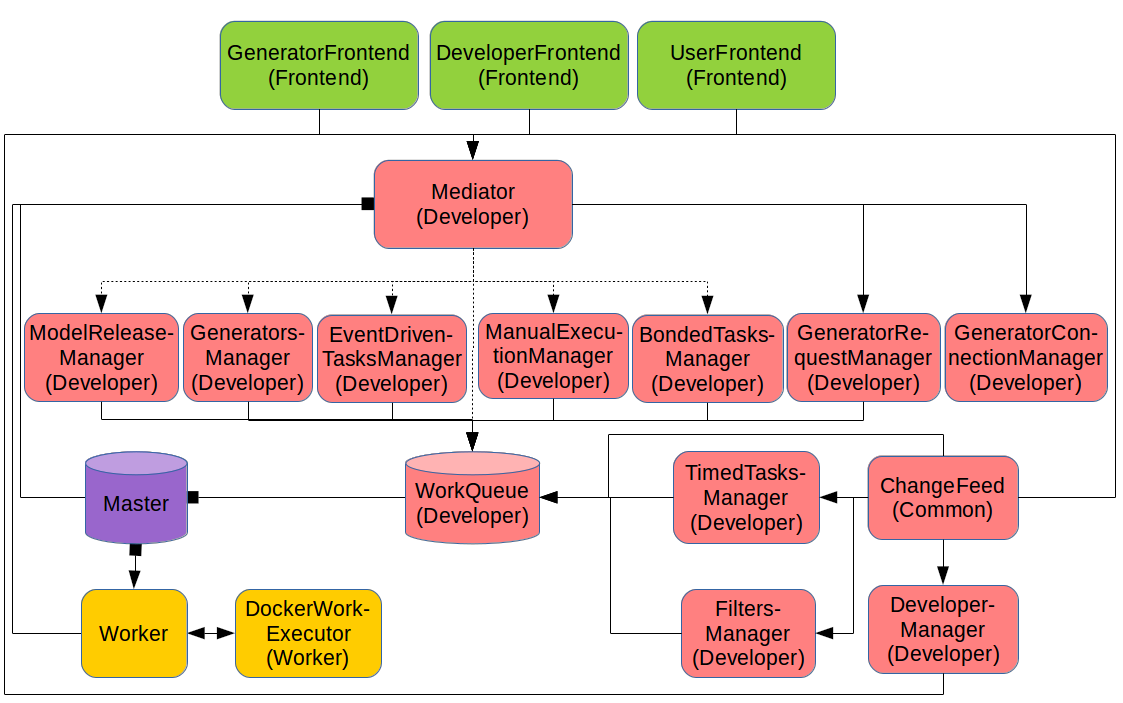
\includegraphics[width=5in]{figures/actor_backend_before.png}
    \caption{Ausgangszustand - Actor Kommunikation}
    \label{fig:ZETA_ACTOR_OLD}
\end{figure}

\begin{sloppypar}
Eine wichtige Funktion der \textit{Akka Actoren} ist ihre Fehlertoleranz \cite{akka_fault_tolerance}. Dabei fungiert ein Actor als \textit{Supervisor} für seine gestarteten Actoren und diese Actoren werden auch Kind Actoren genannt. Somit ergibt sich für die Aktoren zwingend eine hierarchische Struktur, wobei die Actoren auf Exceptions ihrer Kind Actoren reagieren. Die Standard Strategie für Actoren sieht vor, bis auf ein paar Akka interne \textit{Exceptions} den Kind Actor bei einer \textit{Exception} neu zu starten. Alle weiteren Möglichkeiten, wie z.B. ein \textit{Error}, werden auf die nächst höhere Ebene der Hierarchie eskaliert. Die Hierarchie der Actoren in den verschiedenen Diensten des \textit{Actor Clusters} von \textit{Zeta} kann in Abbildung~\ref{fig:ZETA_HIERACHY_OLD} auf Seite~\pageref{fig:ZETA_HIERACHY_OLD} eingesehen werden. Dabei startet z.B. der \textit{Developers} Dienst nur den \textit{Mediator} und den \textit{DeveloperManager} als Top-Level Actor und sämtliche Manager und die \textit{WorkQueue} Actoren werden als Kind Actoren gestartet. Beim \textit{Workers} Dienst wiederum werden alle Actoren als Top-Level Actor gestartet und zusätzlich hat der \textit{Worker} Actor noch eine angepasste \textit{Supervisor Strategy}.
\end{sloppypar}

Ein \textit{Akka Cluster} besteht im Wesentlichen aus \textit{Seed} Nodes und den regurlären \textit{Akka Nodes} \cite{akka_cluster}. Dabei übernehmen die \textit{Seeds} die Aufgabe neue Teilnehmer des Clusters entgegenzunehmen und auch die \textit{Seeds} selbst nutzen die \textit{Seeds} um dem \textit{Akka Cluster} beizutreten. Eine Node ist ein logischer Teilnehmer des Clusters und wird über die Kombination aus Hostname, Port und \textit{UID} identifiziert. Ein \textit{UID} wird einmalig beim Starten einer Node erstellt und verhindert, dass bei einem \textit{Remote Death} eine Node erneut dem Cluster beitreten kann. Das Konzept hinter den Verteilten Workern von \textit{Zeta} basiert auf einem \textit{Worker-Pull} Pattern \cite{akka_worker_pull}. Dabei nehmen die Master die eigentlichen zu bearbeitenden Aufgaben entgegen und die Worker fragen beim Master nach Arbeit. Bei \textit{Zeta} übernimmt der\textit{B1} Dienst zum einen die Aufgabe der \textit{Seed} Node und des Masters. Zusätzlich kommt noch ein \textit{Developers} Dienst zum Einsatz. Innerhalb des \textit{Developers} Dienstes werden sämtliche Anfragen der Websockets des \textit{Play Servers} über die Frontend Actoren entgegen genommen. Dabei wandeln verschiedenen Actoren wie z.B. \textit{GeneratorManager} innerhalb des \textit{Developers} Diensts die Anfragen in sogenannte \textit{Jobs} um und befüllen damit die Warteschlange des \textit{WorkQueue} Actors. Neben den Anfragen aus den Websockets des \textit{Play Servers} nimmt innerhalb des \textit{Developers} Dienstes der \textit{ChangeFeed} Actor Datenbank Änderungen über den \textit{Change Feed} des \textit{Couchbase Sync Gateways} entgegen. Daraufhin sendet der \textit{ChangeFeed} Actor die über den Websocket empfangenen Datenbank Änderungen an sämtliche Actoren des \textit{Developers} Dienstes. Jedoch werden die Nachrichten nur von einem Bruchteil der Actoren auch wirklich verarbeitet und aus diesem Grund sind in Abbildung~\ref{fig:ZETA_ACTOR_OLD} auf Seite~\pageref{fig:ZETA_ACTOR_OLD} auch nur wenige Actoren mit dem \textit{ChangeFeed} Actor verbunden.

\begin{figure}
    \centering
    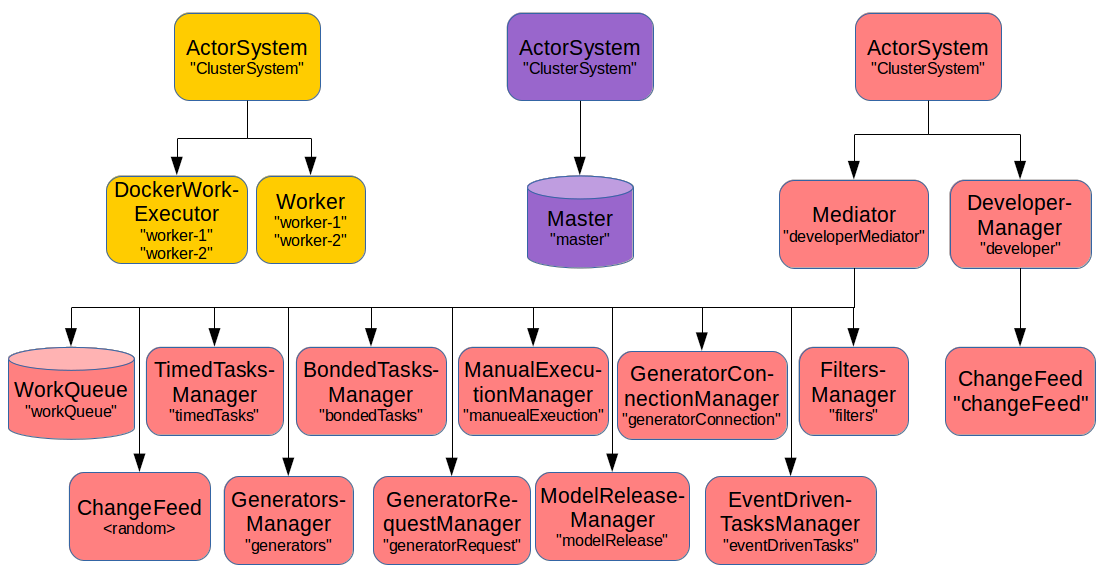
\includegraphics[width=5in]{figures/actor_hierachy_before.png}
    \caption{Ausgangszustand - Actor Hierachie}
    \label{fig:ZETA_HIERACHY_OLD}
\end{figure}

Der \textit{Workers} Dienst ist schlussendlich für die Ausführung der verschiedenen Generatoren per \textit{Docker} zuständig. Dabei wird entsprechend für einen Generator ein neuer \textit{Docker Container} aus den zuvor gebauten \textit{Docker Images} erzeugt und gestartet. Der Generator Container wird beim Start mit in das \textit{Docker Compose} Netzwerk aufgenommen. Mit diesem Zugriff und den übergebenen Parametern wie z.B. dem \textit{Sync Gateway} Sitzungsschlüssel ist der Generator in der Lage, bei der ersten Ausführung sich mit einem Beispiel Programmcode für den entsprechenden Generator zu erstellen. Danach kann der eigentliche Generator in einer separaten Ausführung eines neuen \textit{Docker Containers} ausgeführt werden. Zu diesem Zweck werden innerhalb des Generators über die ID des Generators die Dateien mit den Transformationsregeln von der \textit{Couchbase Datenbank} geladen. Der Inhalt der Dateien wird nun per \textit{Toolbox} des Scala Compilers zur Laufzeit zu einem Transformer kompiliert und mit den Daten einer Modell Instanz ausgeführt. Dabei werde die Daten der Modell Instanz in Form der Datenbank \textit{Entity} an den Transformer übergeben. Grundsätzlich sind die Generatoren in \textit{Zeta} in \textit{Basic-}, \textit{Specific-}, \textit{File-} und \textit{Remote-Generator} unterteilt. Der \textit{Basic-Generator} ist ein vom Meta Modell unabhängiger Generator und der \textit{Specific-Generator} ist für ein bestimmtes Meta Modell. Der \textit{File-Generator} demonstriert das Erstellen von Dateien innerhalb eines Generators und der \textit{Remote-Generator} demonstriert das Ausführen eines weiteren Generators per Websocket vom \textit{Play Server}. Neben diesen Generatoren werden auch der \textit{Filter} und das \textit{MetaModelRelease} vom \textit{Workers} Dienst als eigenständiger \textit{Docker Container} ausgeführt. Beim \textit{Filter} werden in Scala erstellte Regeln zur Filterung der Modell Instanzen wie bei den Generatoren über die Scala \textit{Toolbox} ausgeführt. Das Ergebnis wird zusammen mit dem \textit{Filter} gespeichert. Beim \textit{MetaModelRelease} wird der aktuelle Stand aus \textit{Code-Editor} und \textit{MetaModel-Editor} genommen und unter einer neuen Version abgespeichert.

\subsection{Datenbanken}

Aktuell werden innerhalb von \textit{Zeta} mehrere Datenbanken eingesetzt. Zum einen eine \textit{MongoDB}, aber auch eine \textit{Couchbase Server} mit davor geschaltetem \textit{Sync Gateway}. Beide Datenbank Systeme sind \textit{NoSQL} Datenbanken und arbeiten mit \ac{json} Dokumente. Dabei bieten beide Datenbank Systeme nicht wie z.B. bei relationalen Datenbanken eine offen gehaltene Verbindung, sondern eine über \ac{http} laufende \ac{rest} \acp{api}. Auf der einen Seite wurde die \textit{MongoDB} in der Vergangenheit primär in \textit{Zeta} verwendet. Wie in der Abbildung~\ref{fig:ZETA_ARCH_OLD} auf Seite~\pageref{fig:ZETA_ARCH_OLD} zu sehen ist, wird die \textit{MongoDb} nur vom \textit{Play Server} verwendet und ist nicht öffentlich über den \textit{Proxy} Dienst zugänglich. Inzwischen wird die \textit{Mongodb} innerhalb des \textit{Play Servers} nur noch für die Persistierung der Daten aus dem Websocket des \textit{Code-Editors} verwendet.

Auf der anderen Seite wird die \textit{Couchbase Datenbank} mit dem \textit{Sync Gateway}, wie in Abbildung~\ref{fig:ZETA_ARCH_OLD} auf Seite~\pageref{fig:ZETA_ARCH_OLD} zusehen, von fast allen Diensten innerhalb von \textit{Zeta} verwendet. Zudem erfolgen auch während der Ausführung der Generatoren mehrere Zugriffe auf die Datenbank. Dadurch ist die \textit{Couchbase Datenbank} primär für die Persistierung der angefallenen Daten innerhalb von \textit{Zeta} zuständig. Zum Teil haben die Daten aus dem \textit{Couchbase Server} Überlappungen mit den Daten in der \textit{Mongodb}. Das vor der \textit{Couchbase Datenbank} geschaltete \textit{Sync Gateway} ist zusätzlich auch öffentlich über den \textit{Proxy} Dienst erreichbar. Dieser externe Zugriff auf das \textit{Sync Gateway} wird dazu genutzt um vom Browser aus innerhalb der \textit{Webbapp} auf die Datenbank zuzugreifen. Speziell der \textit{Change Feed} des \textit{Sync Gateways} wird einmal innerhalb der \textit{Webapp} im Browser und zudem mehrfach von den Actoren des \textit{Akka Clusters} des \textit{Backend} Projekts genutzt.

